\documentclass[aspectratio=169,11pt]{beamer}

\usepackage[T1]{fontenc}
\usepackage[utf8]{inputenc}
\usepackage[spanish,es-noquoting,es-nolists,es-noshorthands]{babel}
\usepackage{lmodern}
\usepackage{amsmath,amssymb}
\usepackage{booktabs}
\graphicspath{{figuras/}{../entrega-final/figuras/}}

\usetheme{default}
\usecolortheme{default}
\definecolor{tinta}{HTML}{1F2933}
\definecolor{acento}{HTML}{2A78D6}
\definecolor{suave}{HTML}{6B7280}
\setbeamercolor{frametitle}{fg=tinta}
\setbeamercolor{title}{fg=tinta}
\setbeamercolor{structure}{fg=acento}
\setbeamercolor{normal text}{fg=tinta}
\setbeamerfont{frametitle}{series=\bfseries,size=\Large}
\setbeamertemplate{navigation symbols}{}
\setbeamertemplate{itemize items}{\color{acento}\textbullet}
\setbeamertemplate{footline}{\hfill{\color{suave}\scriptsize\insertframenumber/\inserttotalframenumber}\hspace{1em}\vspace{0.6em}}
\newcommand{\clave}[1]{{\color{acento}\bfseries #1}}

\title{Estructura frente a tamaño}
\subtitle{Selección de conjuntos críticos en el grafo de exposición de DeFi}
\author{David Sánchez Lombana \and Juan Sebastián Cuesta Montenegro}
\institute{Teoría de Grafos 2026-II · Prof.\ Daniel Bojacá\\Universidad del Rosario}
\date{Noviembre de 2026}

\begin{document}

\begin{frame}
\titlepage
\end{frame}

\begin{frame}{Motivación}
\begin{itemize}
\item Los protocolos DeFi reutilizan los mismos activos como colateral: la
      caída de uno se propaga a los que dependen de él.
\item Eso induce un \clave{grafo dirigido y ponderado de exposición}. DeXposure
      (Wu \emph{et al.}, 2025) ya lo construyó: 314 semanas, 2018--2024.
\item El estado del arte elige qué protocolos estresar \clave{por tamaño}: el
      mayor, los cinco mayores, un sector.
\end{itemize}
\vspace{1em}
\begin{block}{Pregunta}
Con un presupuesto de $k$ protocolos, ¿qué conjunto fragmenta más la red? ¿Lo
encuentran mejor los criterios estructurales o los de tamaño?
\end{block}
\end{frame}

\begin{frame}{El problema}
\begin{itemize}
\item $G_t=(V_t,E_t,w_t)$: $u\to v$ si $u$ depende de $v$, con peso en USD.
\item Proyección no dirigida y componente gigante $C_t$; se trabaja en
      $H_t=\tilde G_t[C_t]$ (98--99{,}8\,\% de los vértices).
\item Dado $k$, hallar $S\subseteq C_t$, $|S|=k$, que minimice lo que queda
      conectado. Es \clave{NP-duro} (interdicción de vértices): heurísticas.
\end{itemize}
\vspace{0.6em}
\textbf{Dos medidas de daño}, porque contar protocolos y medir exposición no
coinciden:
\[
R_{\mathrm{est}}=\frac{\max_Q|Q|}{|C_t|},\qquad
R_{\mathrm{pond}}=\frac{\max_Q W_t(Q)}{W_0},\qquad L=1-R
\]
\[
L_{\mathrm{pond}}=\underbrace{L_{\mathrm{directa}}}_{\text{peso de }S}
+\underbrace{L_{\mathrm{frag}}}_{\text{peso desconectado}}
\]
\end{frame}

\begin{frame}{Seis reglas en competencia}
\begin{columns}[T]
\column{0.5\textwidth}
\textbf{Tamaño}
\begin{itemize}
\item Fuerza de exposición (suma de pesos)
\item PageRank dirigido y ponderado
\end{itemize}
\vspace{0.5em}
\textbf{Estructura}
\begin{itemize}
\item Intermediación
\item Articulación adaptativa
\item CDS de Guha--Khuller + voraz dentro
\item Inmunización espectral exacta
\end{itemize}
\column{0.5\textwidth}
\textbf{Controles}
\begin{itemize}
\item Voraz sin restricción sobre $L_{\mathrm{pond}}$
\item 20 permutaciones aleatorias
\item TVL y SIS de DeXposure-FM (solo exploratorio)
\end{itemize}
\vspace{0.5em}
\textbf{Protocolo}
\begin{itemize}
\item 13 semanas fijadas de antemano: un trimestre 2022--2024 + previas a
      Terra, FTX y USDC
\item $k\in\{1,2,5,10,20\}$
\end{itemize}
\end{columns}
\end{frame}

\begin{frame}{Implementación: \texttt{critset}}
\begin{itemize}
\item Paquete Python (uv): NumPy, SciPy, igraph. CLI \texttt{run},
      \texttt{experiment}, \texttt{case}, \texttt{characterize}, \texttt{plots}.
\item \clave{Articulación} en $O(n+m)$ por paso: Tarjan con tamaños de
      subárbol da la pieza mayor tras quitar cada vértice.
\item \clave{Espectral exacta} y barata: $\rho(A)=\max_{\text{SCC}}\rho(A[\text{SCC}])$,
      así que solo se evalúan los vértices de la SCC dominante (393--1\,230 de
      1\,058--2\,838).
\item Evaluación del daño vectorizada; experimento paralelo y reanudable.
\item \clave{48 pruebas} contra NetworkX y fuerza bruta: medidas de daño,
      articulación, validez del CDS, PageRank, regla espectral, 2-núcleo.
\end{itemize}
\end{frame}

\begin{frame}{Resultado 1: los dos objetivos ordenan al revés}
\centering
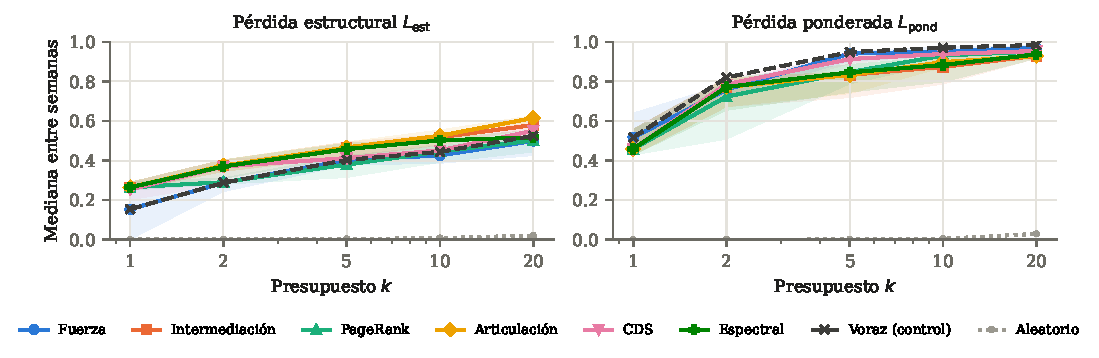
\includegraphics[width=\textwidth]{fig_curvas.pdf}

\small Mediana de 13 semanas; banda: rango intercuartílico.
\end{frame}

\begin{frame}{Resultado 1: cada familia gana en lo que optimiza}
\centering
\small
\begin{tabular}{lcccccc}
\toprule
& \multicolumn{2}{c}{$L_{\mathrm{est}}$} & \multicolumn{2}{c}{$L_{\mathrm{pond}}$} & \multicolumn{2}{c}{$F_{\mathrm{rel}}$} \\
Regla & med. & gana & med. & gana & med. & gana \\
\midrule
Fuerza          & 0{,}43 & 0/0  & 0{,}95 & 0/7  & 0{,}011 & 0/8 \\
Intermediación  & 0{,}52 & 1/9  & 0{,}87 & 0/0  & 0{,}009 & 1/7 \\
PageRank        & 0{,}45 & 0/0  & 0{,}93 & 0/0  & 0{,}010 & 1/7 \\
Articulación    & \textbf{0{,}53} & \textbf{13/13} & 0{,}90 & 0/0 & 0{,}010 & 1/8 \\
CDS             & 0{,}45 & 0/0  & 0{,}94 & 0/4  & 0{,}016 & 3/10 \\
Espectral       & 0{,}50 & 0/0  & 0{,}88 & 0/0  & 0{,}016 & 0/8 \\
Voraz (control) & 0{,}44 & 0/0  & \textbf{0{,}97} & \textbf{13/13} & 0{,}016 & 7/10 \\
\midrule
Aleatorio       & 0{,}01 & --   & 0{,}01 & --   & 0{,}000 & -- \\
\bottomrule
\end{tabular}

\vspace{0.3em}
{\footnotesize $k=10$, mediana de 13 semanas; gana = semanas estrictas / a menos de 0{,}01 del máximo.}
\begin{itemize}
\item Articulación optimiza $R_{\mathrm{est}}$; el voraz, $L_{\mathrm{pond}}$: \clave{victorias en parte circulares}.
\item Articulación vs.\ intermediación: $+0{,}012$ (IC 95\,\%: 0{,}007--0{,}017), empate práctico.
\item CDS queda 0{,}020 bajo el voraz: su mérito es el voraz, no la columna vertebral.
\item $F_{\mathrm{rel}}$, que nadie optimiza: \clave{ninguna familia domina}.
\end{itemize}
\end{frame}

\begin{frame}{Resultado 2: de qué está hecho el daño}
\centering
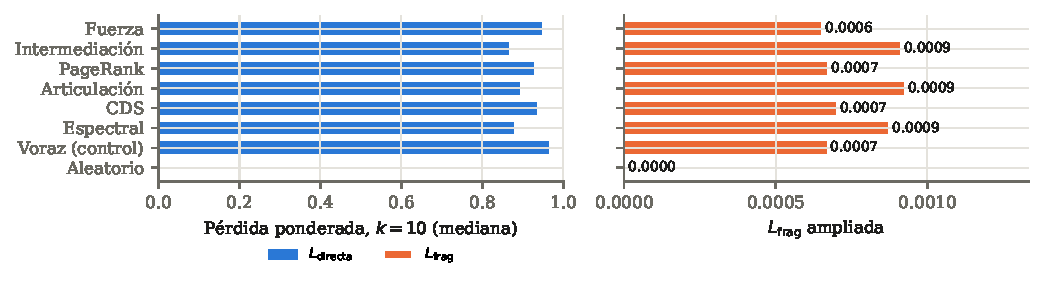
\includegraphics[width=\textwidth]{fig_descomposicion.pdf}

\vspace{0.3em}
\begin{itemize}
\item $L_{\mathrm{frag}}\le 0{,}009$ en todo conjunto evaluado: la exposición se pierde \clave{quitando}, no partiendo.
\item Articulación: 84\,\% de su $L_{\mathrm{est}}$ son \clave{hojas aisladas}.
\item En fragmentos $\geq2$: 0{,}08 (articulación) vs.\ 0{,}05 (fuerza). Ventaja real, pero de 3 puntos.
\end{itemize}
\end{frame}

\begin{frame}{Resultados teóricos}
\begin{itemize}
\item \clave{Lema de las hojas.} Para ambos objetivos existe un óptimo sin hojas
      (intercambio hoja $\to$ vecino). Reduce la búsqueda en 37--45\,\%.
\item \clave{Articulación es óptima para $k=1$} en $L_{\mathrm{est}}$: un no-corte deja $n-1$; un corte, a lo sumo $n-2$.
\item \clave{$L_{\mathrm{directa}}$ es submodular}: cobertura ponderada de aristas.
      El voraz garantiza $(1-1/e)$ y, para $k=1$, la fuerza es óptima.
      Con $L_{\mathrm{frag}}\approx0$, explica por qué el tamaño gana en exposición.
\item \clave{Atajo espectral}: $\rho(A)=\max_{\text{SCC}}\rho$ (forma normal de Frobenius);
      solo la SCC dominante importa, y con empate ninguna remoción baja $\rho$.
\item \clave{Tarjan}: un DFS da la componente mayor tras quitar cada punto de articulación, en $O(n+m)$.
\end{itemize}
\end{frame}

\begin{frame}{Resultado 3: sensibilidad}
\centering
\small
\begin{tabular}{lccc}
\toprule
$k=10$, $L_{\mathrm{est}}$ / $L_{\mathrm{pond}}$ & Sin \emph{Unknown} & Sin no protocolos & 2-núcleo \\
\midrule
Fuerza         & 0{,}21 / 0{,}92 & 0{,}11 / 0{,}69 & 0{,}22 / 0{,}96 \\
Intermediación & 0{,}36 / 0{,}81 & 0{,}28 / 0{,}55 & 0{,}28 / 0{,}85 \\
PageRank       & 0{,}28 / 0{,}82 & 0{,}19 / 0{,}56 & 0{,}21 / 0{,}95 \\
Articulación   & \textbf{0{,}38} / 0{,}83 & \textbf{0{,}30} / 0{,}51 & \textbf{0{,}30} / 0{,}90 \\
CDS            & 0{,}25 / 0{,}90 & 0{,}22 / 0{,}75 & 0{,}21 / 0{,}90 \\
Voraz          & 0{,}24 / \textbf{0{,}94} & 0{,}19 / \textbf{0{,}77} & 0{,}22 / \textbf{0{,}97} \\
\bottomrule
\end{tabular}

\vspace{0.6em}
\raggedright
\begin{itemize}
\item \emph{Unknown}: contrapartes no identificadas, adyacente al 63--74\,\% de $C_t$.
\item No protocolos: \emph{Unknown} + 8 cadenas + 15 exchanges centralizados.
\item 2-núcleo: sin hojas, 54--61\,\% de $C_t$. La ventaja estructural \clave{persiste, más chica}.
\end{itemize}
\end{frame}

\begin{frame}{Resultado 4: dos familias de conjuntos}
\begin{columns}[c]
\column{0.5\textwidth}
\centering
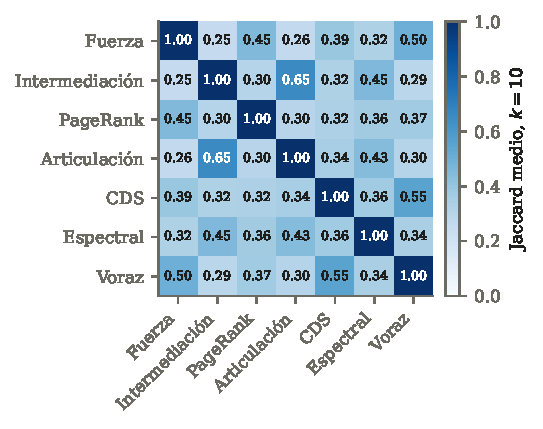
\includegraphics[width=\textwidth]{fig_jaccard.pdf}
\column{0.5\textwidth}
\begin{itemize}
\item El conjunto estructuralmente crítico \clave{no} es el de los más grandes:
      Jaccard fuerza--articulación 0{,}26.
\item Las estructurales se parecen entre sí (0{,}65).
\item El voraz se parece al CDS (0{,}55) y a la fuerza (0{,}50).
\end{itemize}
\end{columns}
\end{frame}

\begin{frame}{Episodios y controles de tamaño}
\textbf{Estudio de caso (Terra/Luna, FTX, USDC)}
\begin{itemize}
\item Indicador fijado antes: caída de al menos 50\,\% de la fuerza en 4 semanas.
\item Tasa base de 47--67\,\%: recoge la caída general de precios.
\item Con $k=10$ ninguna regla supera la tasa base en los tres episodios.
      \clave{Resultado nulo}; falta una lista curada de afectados.
\end{itemize}
\vspace{0.5em}
\textbf{TVL y SIS}
\begin{itemize}
\item El TVL publicado falta para el 13--22\,\% de $C_t$ (21--49\,\% de la fuerza).
\item Con faltantes en cero ($k=10$): TVL retira 0{,}52--0{,}67 y SIS 0{,}62--0{,}91, frente a 0{,}90--0{,}95 de la fuerza. Solo exploratorio.
\end{itemize}
\end{frame}

\begin{frame}{Costo computacional}
\begin{columns}[c]
\column{0.5\textwidth}
\centering
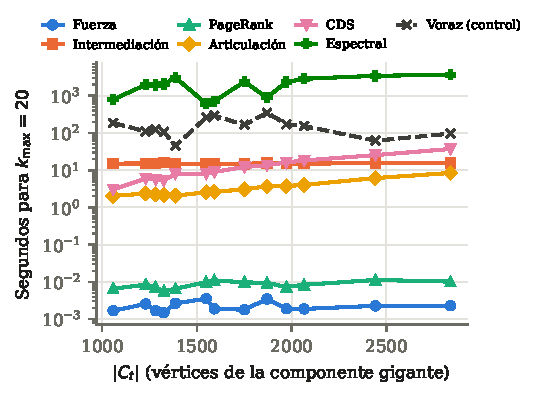
\includegraphics[width=\textwidth]{fig_tiempos.pdf}
\column{0.5\textwidth}
\begin{itemize}
\item Fuerza y PageRank: milisegundos.
\item Articulación: 2--8\,s. CDS: 3--37\,s.
\item Intermediación: $\approx$15\,s. Voraz: 45--350\,s.
\item Espectral exacta: la más cara (hasta $\approx$1\,h con $k=20$ y 13
      semanas en paralelo).
\item Todas viables para monitoreo semanal.
\end{itemize}
\end{columns}
\end{frame}

\begin{frame}{Conclusiones}
\begin{itemize}
\item Articulación gana en protocolos desconectados; el voraz, en exposición.
      \clave{Cada uno gana en lo que optimiza.}
\item El daño estructural es sobre todo \clave{aislar hojas}; la ventaja en fragmentos reales existe pero es pequeña.
\item Con $F_{\mathrm{rel}}$, que nadie optimiza, \clave{ninguna regla parte la exposición}: en promedio queda más del 94\,\% en una componente.
\item La submodularidad de $L_{\mathrm{directa}}$ explica por qué el tamaño gana en exposición.
\item Robusto sin \emph{Unknown}, sin cadenas ni exchanges y en el 2-núcleo.
\end{itemize}
\vspace{0.5em}
\textbf{Pendiente}: modelo nulo con recableado, reglas adaptativas y de desmantelamiento,
óptimo exacto para $k=2$, alcance dirigido o DebtRank, episodios normalizados por mercado.
\end{frame}

\begin{frame}
\centering
\vfill
{\Large\bfseries ¡Gracias!}

\vspace{1em}
{\color{suave} Herramienta, datos y resultados: \texttt{critset-herramienta.zip}}
\vfill
\end{frame}

\end{document}
